\documentclass[14pt]{extarticle}

\usepackage{fancyhdr,amsfonts,graphicx,wrapfig,sidecap,float,adjustbox,subcaption,indentfirst,amsmath}

\usepackage[right=2.5cm,left=2.5cm,top=2.5cm,bottom=2.5cm]{geometry}

\lstset{frame=tb,
	language=Java,
	aboveskip=3mm,
	belowskip=3mm,
	showstringspaces=false,
	columns=flexible,
	basicstyle={\small\ttfamily},
	numbers=none,
	numberstyle=\tiny\color{gray},
	keywordstyle=\color{blue},
	commentstyle=\color{dkgreen},
	stringstyle=\color{mauve},
	breaklines=true,
	breakatwhitespace=true,
	tabsize=3
}
\pagestyle{fancy}
\lhead{Memorial University of Newfoundland}
\rhead{Department of Mathematics and Statistics}
\renewcommand{\headrulewidth}{0.4pt}

\lfoot{Mathematics 2130}
\cfoot{}
\rfoot{Fall 2015, Project 1}
\renewcommand{\footrulewidth}{0.4pt}

\begin{document}
\begin{titlepage}
\vspace*{2in}
\begin{center}
{\LARGE Quadratic and Cubic Formula}
\end{center}

\vspace{2cm}

\abstract{This paper explains the mechanics of the Quadratic and Cubic formulae. Graphical analysis of these equations, shows what these formulae represent and the importance of the discriminant in the equations. }


\vspace{3in}
\begin{flushright}
\begin{tabular}{l}
Project 1 \\
Mathematics 2130\\
Submitted by: John Hollett\\
Submitted to: Ivan Booth\\
\today
\end{tabular}
\end{flushright}


\end{titlepage}


\lhead{Quadratic and Cubic Formulae}
\rhead{Math 2130}
\lfoot{John Hollett}
\rfoot{\thepage}
%\underheadoverfoot




\section{Introduction}
Quadratic and cubic formulae are used in many fields of mathematics and some of these include: Physics, Chemistry, Engineering, etc. They are used to find the roots or x-values in an equation such that it is equal to zero based on it's constants. When being applied to fields in math, such as physics, it can be used to find projectile motions. In Chemistry it is used to find equilibrium in chemical equations. The formulae below are used in this paper to determine their properties and examine them graphically. The discriminant of each formula is an attribute of itself and is meaningless on it's own.


\begin{equation}
	\text{Quadratic Formula} \to ax^2+bx+c=0
	\label{E1}
\end{equation}
\begin{equation}
	\text{Cubic Formula} \to x^3+bx+c=0
	\label{E2}
\end{equation}

\begin{equation}
	\text{Quadratic Discriminant} \to b^2-4ac
	\label{E3}
\end{equation}
\begin{equation}
	\text{Cubic Discriminant} \to 4b^3+27c^2
	\label{E4}
\end{equation}

\section{The Constants of the Quadratic Formula}
\subsection{Basic Analysis}
In reference to Equation (\ref{E1}), there are three coefficients ($a$,$b$ and $c$) that are used. When using either formula, an equation following with constant coefficients is necessary. Either quadratic or cubic formula will fail if this requirement is not satisfied from the start.

\indent Each of the constants affects the root(s) for each respective quadratic equation used. When using Formula (\ref{E1}) to solve for the roots of an equation, it will yield two results. If the discriminant is positive, it will yield two Real roots such as Figure (\ref{fig:img3}). If the discriminant is negative, it will yield two imaginary roots like Figure (\ref{fig:img2}). Otherwise, the discriminant is zero and the result is one root as shown in Figure (\ref{fig:img1}). These are the only possible cases for the quadratic formula. In comparison, the cubic formula has three cases with completely different implications. If the discriminant is positive, there is one real and two imaginary roots; if it is negative there are three real roots; it is zero, there are three real roots in which two are equal and one is not.
\footnotesize
\begin{figure}[h]
\caption{Curve Examples}
\begin{subfigure}{0.33\textwidth}
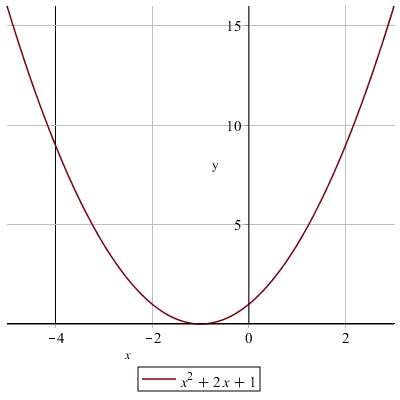
\includegraphics[width=0.8\linewidth]{graph1.png}
\caption{One X-Value}
\label{fig:img1}
\end{subfigure}
\begin{subfigure}{0.33\textwidth}
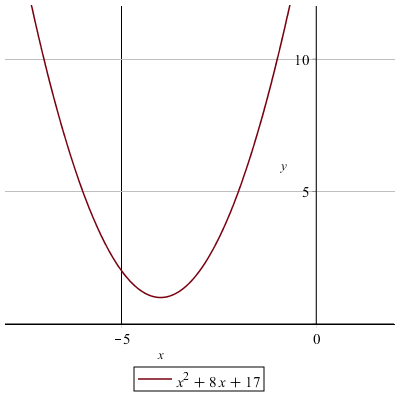
\includegraphics[width=0.8\linewidth]{graph2.png}
\caption{Two Imaginary X-Values}
\label{fig:img2}
\end{subfigure}
\begin{subfigure}{0.33\textwidth}
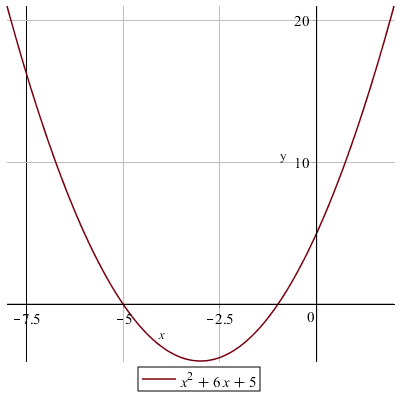
\includegraphics[width=0.8\linewidth]{graph3.png}
\caption{Two Real X-Values}
\label{fig:img3}
\end{subfigure}
\end{figure}
\normalsize

The three of these curves are indicative of the three cases the discriminant of the quadratic formula presents. Even with imaginary roots, this is not an undesired result, as shown by Figure (\ref{fig:img2}), the graph still exists, therefore imaginary numbers do not change things very much.
\subsubsection{The Constant $a$}
\indent The Quadratic Equation (\ref{E1}) has a constant $a$, which affects the roots in solving the equation for the respective problem. Although this does not affect it too drastically, it still has an impact that is scalar. For example: $$ (2x^2+12x+18) = 2(x^2+6x+9) = 2(x+3)(x+3) = 2(x+3)^2$$
\indent Using the above example, it is evident that the constant $a$ acts as a scalar for the equation. It is like the difference between $y=2x$ and $y=3x$; they have a steeper slope. For the purpose of this paper, we will factor it out and represent it as:
$$\frac{1}{a}(ax^2+bx+c) = \frac{ax^2}{a}+\frac{bx}{a}+\frac{c}{a} = x^2+\frac{b}{a}x+\frac{c}{a} $$
\indent Finally, using the above result, we can substitute $\frac{b}{a} = B $ and $\frac{c}{a} = C$ and apply this to the formula below we can derive a new equation:
\begin{equation}
x^2+Bx+C=0
\label{E5}
\end{equation}
\indent Using Equation (\ref{E5}), all calculations are done assuming $a=1$ to simplify this the equation. This is with respect to the above assumption made; it does not affect the equation as much as the other quantities. The only exception to this is when $a\geq\frac{b^2}{4c}$. This will never happen because the value $a=1$ is used for every analysis from here on forward.
\subsubsection{The Constants $B$ and $C$}

\indent The newly derived equation using $B$ and $C$ will be used to examine the quadratic formula. These values will affect the discriminant in Equation (\ref{E3}) the most for the purpose of this paper. But, in order to understand what is happening in more detail, we will first need to solve for $x$.

$$x^2+Bx+C=0 \to x^2+Bx=-C\to x^2+Bx+(\frac{B}{2})^2=-C+(\frac{B}{2})^2$$
$$(x+\frac{B}{2})^2 = \frac{B^2}{4}-C = \frac{B^2-4C}{4}\to \sqrt{(x+\frac{B}{2})^2}=\pm\sqrt{\frac{B^2-4C}{4}} \to x+\frac{B}{2} = \pm\frac{\sqrt{B^2-4C}}{2}$$
\begin{equation}
x=\frac{-B\pm\sqrt{B^2-4C}}{2}
\label{E6}
\end{equation}
\begin{figure}[h]
\begin{subfigure}{0.50\textwidth}
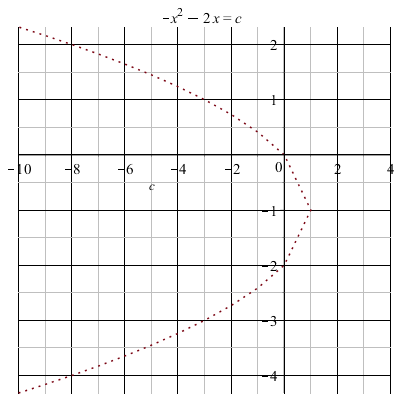
\includegraphics[scale=0.58]{graph10.png}
\caption{\small$C$ as a function of $x$}
\label{fig:img10}
\end{subfigure}
\begin{subfigure}{0.50\textwidth}
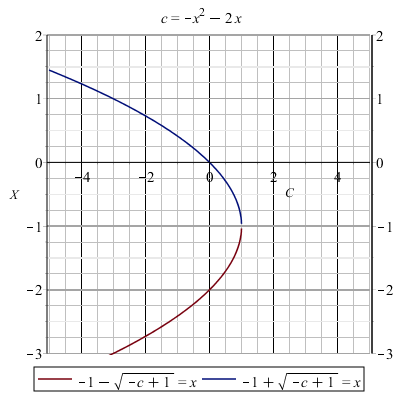
\includegraphics[scale=0.58]{graph4.png}
\caption{\small$C$ as a function of $x$}
\label{fig:img4}
\end{subfigure}
\end{figure}

\normalsize
\indent The above Equation (\ref{E6}) is solved for $x$ instead of $zero$ as in Equation (\ref{E1}) above. This is important because now if we want to know any roots, all we have to do is substitute in $B$ and $C$ into the above Equation (\ref{E6}) and we can find them right away (at least when $a=1$). The only issue with this is for imaginary solutions we have to make sure the software being used can handle impossible mathematical functions such as $\sqrt{-1}$.

We have two curves, blue and the other red. The blue curve indicates one solution of $x$. The red curve indicates a different solution for $x$. This is related to the $\pm$ symbol of Equation(\ref{E6}). It says there are two solutions and these curves show both of these visually. When they intersect at the vertex point, it produces one root with a multiplicity of two. (For Example: $(x-2)^2=0, x={2}$).

In Figure (\ref{fig:img4}), the graph represents values of $C$. By examination, $C$ does not contain any values very far to the right side of the graph. However, to the left side of the graph, there are many values of $C$ that have two roots.

This is the significance of the discriminant in Equation (\ref{E3}). If we take $C=1$, where the two curves meet, we get equation $x^2+2x+1=0$. If we take $C=0$, we get the equation $x^2+2x=0$. Lastly, with some \textit{imagination}, if we take $C=2$ we get the equation $x^2+2x+2$. If we solve these, we can relate it to the graph.

\indent Taking the equations yielded from the graph thus far, we can solve them and use them to prove our graph.
$$x^2+2x+1=0 \to (x+1)^2=0, x=\{-1\}$$
$$x^2+2x=0 \to x(x+2)=0, x=\{-2,0\}$$
$$x^2+2x+2=0 \to (x+(1+i))(x+(1-i))=0, x=\{-1+i,-1-i\}$$
\begin{wrapfigure}[17]{l}{0.425\textwidth}
	\begin{center}
		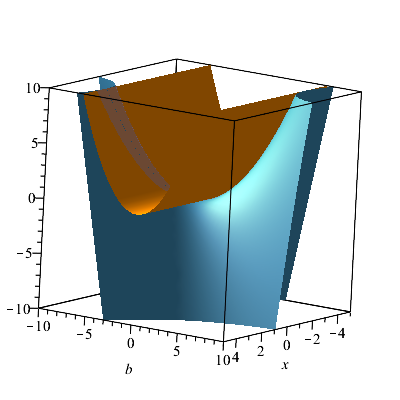
\includegraphics[scale=0.55]{graph8.png}
		\caption{$C$ and $B$ for $x$}
		\label{fig:img5}
	\end{center}
\end{wrapfigure}

\indent If we compare these results to the graph, it can be seen that the roots for these equations line up for these values of $A$,$B$ and $C$ that have been chosen from the graph above. If we take it one step further, we should ask what happens when we adjust $B$ and $C$ from Equation (\ref{E6}) at the same time on a graph.

\indent In Figure (\ref{fig:img5}), we have a planar surface representing values of $B$ and $C$. If we were to pick values of $B$ and $C$, the roots of the equation would match the planar surface represented in the figure.

\indent The surface of the saddle curve is, much like the previous graphs, except it tells reveals more about what is happening. As $B$ and $C$ values are picked for constants, depending on what they are, we can see a pattern. When there is one root, the two values of $B$ and $C$ are along the vertex of the saddle. The sides of the saddle represent the two roots of $x$ as they change. However, what we cannot see from either of the graphs is values representing curves with imaginary discriminants.

\indent An important detail to note about this graph is the orange surface sitting on top of the blue one. This represents the discriminant sliding through the saddle. The reason this is significant is because it shows us the how closely related the discriminant is in determining the roots of any quadratic equation. When the discriminant is alone, it represents a parabolic curve. When the full equation is used, it represents the blue surface.


\indent Despite having many values that would be imaginary in nature, we can assume open space has an imaginary solution that we cannot see. The complex plane contains the imaginary values we cannot see.



\indent By examining Figure (\ref{fig:img5}), we can see a definitive pattern of similarities in the quadratic formula. The shapes we have examined are parabolic in nature. The majority of all the data examined thus far have been with the quadratic formulae. Based on the patterns that are evident in the quadratic formula, the least expected would be three roots for a cubic equation instead of two.

\begin{wrapfigure}[14]{l}{0.425\textwidth}
	\begin{center}
		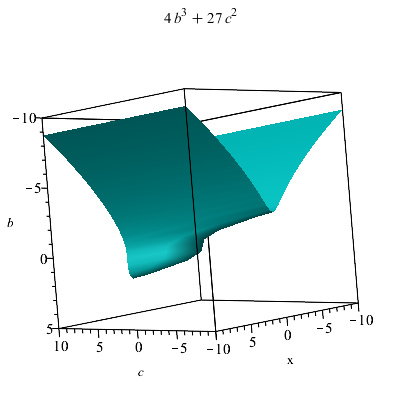
\includegraphics[scale=0.50]{graph6.png}
		\caption{\small Cubic discriminant}
		\label{fig:img7}
	\end{center}
\end{wrapfigure}
Until now, we have only examined the quadratic formula and it's discriminant as well as clear differences between the two. Reiterating, the cubic formula has three roots which are dependent on the discriminant of the cubic formula (See Equation (\ref{E4})). However, it should be noted that the actual cubic formula is different than the one we are looking at. The regular cubic formula is $ax^3+bx^2+cx+d=0$.

\section{The Cubic Formula}
Here we consider the depressed cubic equation $x^3+bx+c=0$ (\ref{E2}). But, all assumptions that are made for quadratics, can be transferred to the basic cubic formula. The cost of this is more effort required and a few minor details.

\subsection{Constants $b$ and $c$ for the Cubic Formula}


As was determined above, the constant $a$ was dropped to simplify the quadratic equation and by now it is evident that the cubic formula will behave the same.

In the quadratic formula, when we used $B$ and $C$ to describe the simplified quadratic formula that was derived by assuming $a=1$, we are using the same assumption here. Much like the quadratic formula, we are still working two constants $b$ and $c$ into the depressed cubic formula.
\begin{wrapfigure}[19]{r}{0.425\textwidth}
	\begin{center}
		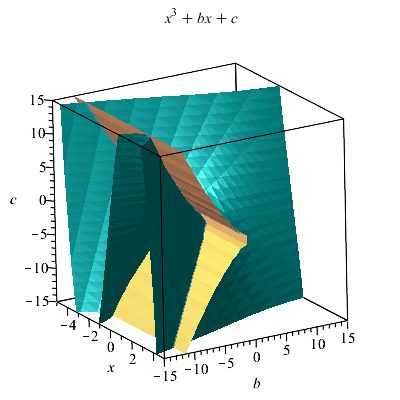
\includegraphics[scale=0.60]{graph9.png}
		\caption{\small Cubic Formula with its discriminant}
		\label{fig:img7}
	\end{center}
\end{wrapfigure}
\indent The discriminant of the cubic formula as seen in Figure (\ref{fig:img7}), looks similar to a cubic curve graphed in 2D. It has a stretched out S-Shape. It shows us the kinds of solutions we can expect when $c=0$ and by is free or vice versa.

\indent In Figure (\ref{fig:img7}), we have the cubic formula graphed in 3D. It is in the shape of a sideways S, except it has depth. To determine what is going on graphically, we will need to make some assumptions based on what was analyzed from quadratic roots.

\indent When examining the $x$-axis in the graph, we can see that if we were to do a line test, the number of times we intersect gives us the real roots we can have for appropriate values of $B$ and $C$.

Three intersections yield three real roots. One intersection and a vertex, will yield us two real roots and one imaginary. A single intersection will always produce one real root and two imaginary roots. And exactly like the quadratic formula, if we have values we would like to try, these surfaces will plot the solutions for us with the assumption $a=1$.

The discriminant is vastly different however. Despite this, just like with quadratics, it slips in around the curves of the cubic surface to support what was found from graphing quadratics. Naturally, this makes sense and we should accept this is not a coincidence and supports what we know. This discriminant is an important aspect that determines the roots.

\section{Conclusion}
Analysis the provided has shown there were similarities and patterns present. The requirement of using either formula to solve a problem, is finding the discriminant. Without the discriminant, the equation is impossible to solve and find. These formulae are the result of mathematicians trying countless techniques to solve for $x$ such that the constant coefficients can be used directly into the equation to find it's roots. Without these equations, many of our proofs in mathematics would be rendered useless.



\newpage

\begin{thebibliography}{99}

\bibitem{wikipedia}"Cubic Function" Wikipedia: The Free Encyclopedia. Wikimedia Foundation, Inc. 10 Sept 2015. Web. 29 Sept 2015

\bibitem{wikipedia}"Quadratic Function" Wikipedia: The Free Encyclopedia. Wikimedia Foundation, Inc. 21 Sept 2015. Web. 28 Sept 2015

\end{thebibliography}


\end{document}
